\documentclass{csse4400}

% \teachermodetrue

\usepackage{float}

\usepackage{languages}

\title{TLDR of Databases in Applications}
\author{Evan Hughes \& Brae Webb}

\date{\week{2}}
\begin{document}

\maketitle

\begin{figure}[h]
  \href{https://www.oreilly.com/library/view/designing-data-intensive-applications/9781491903063/ch02.html}{
    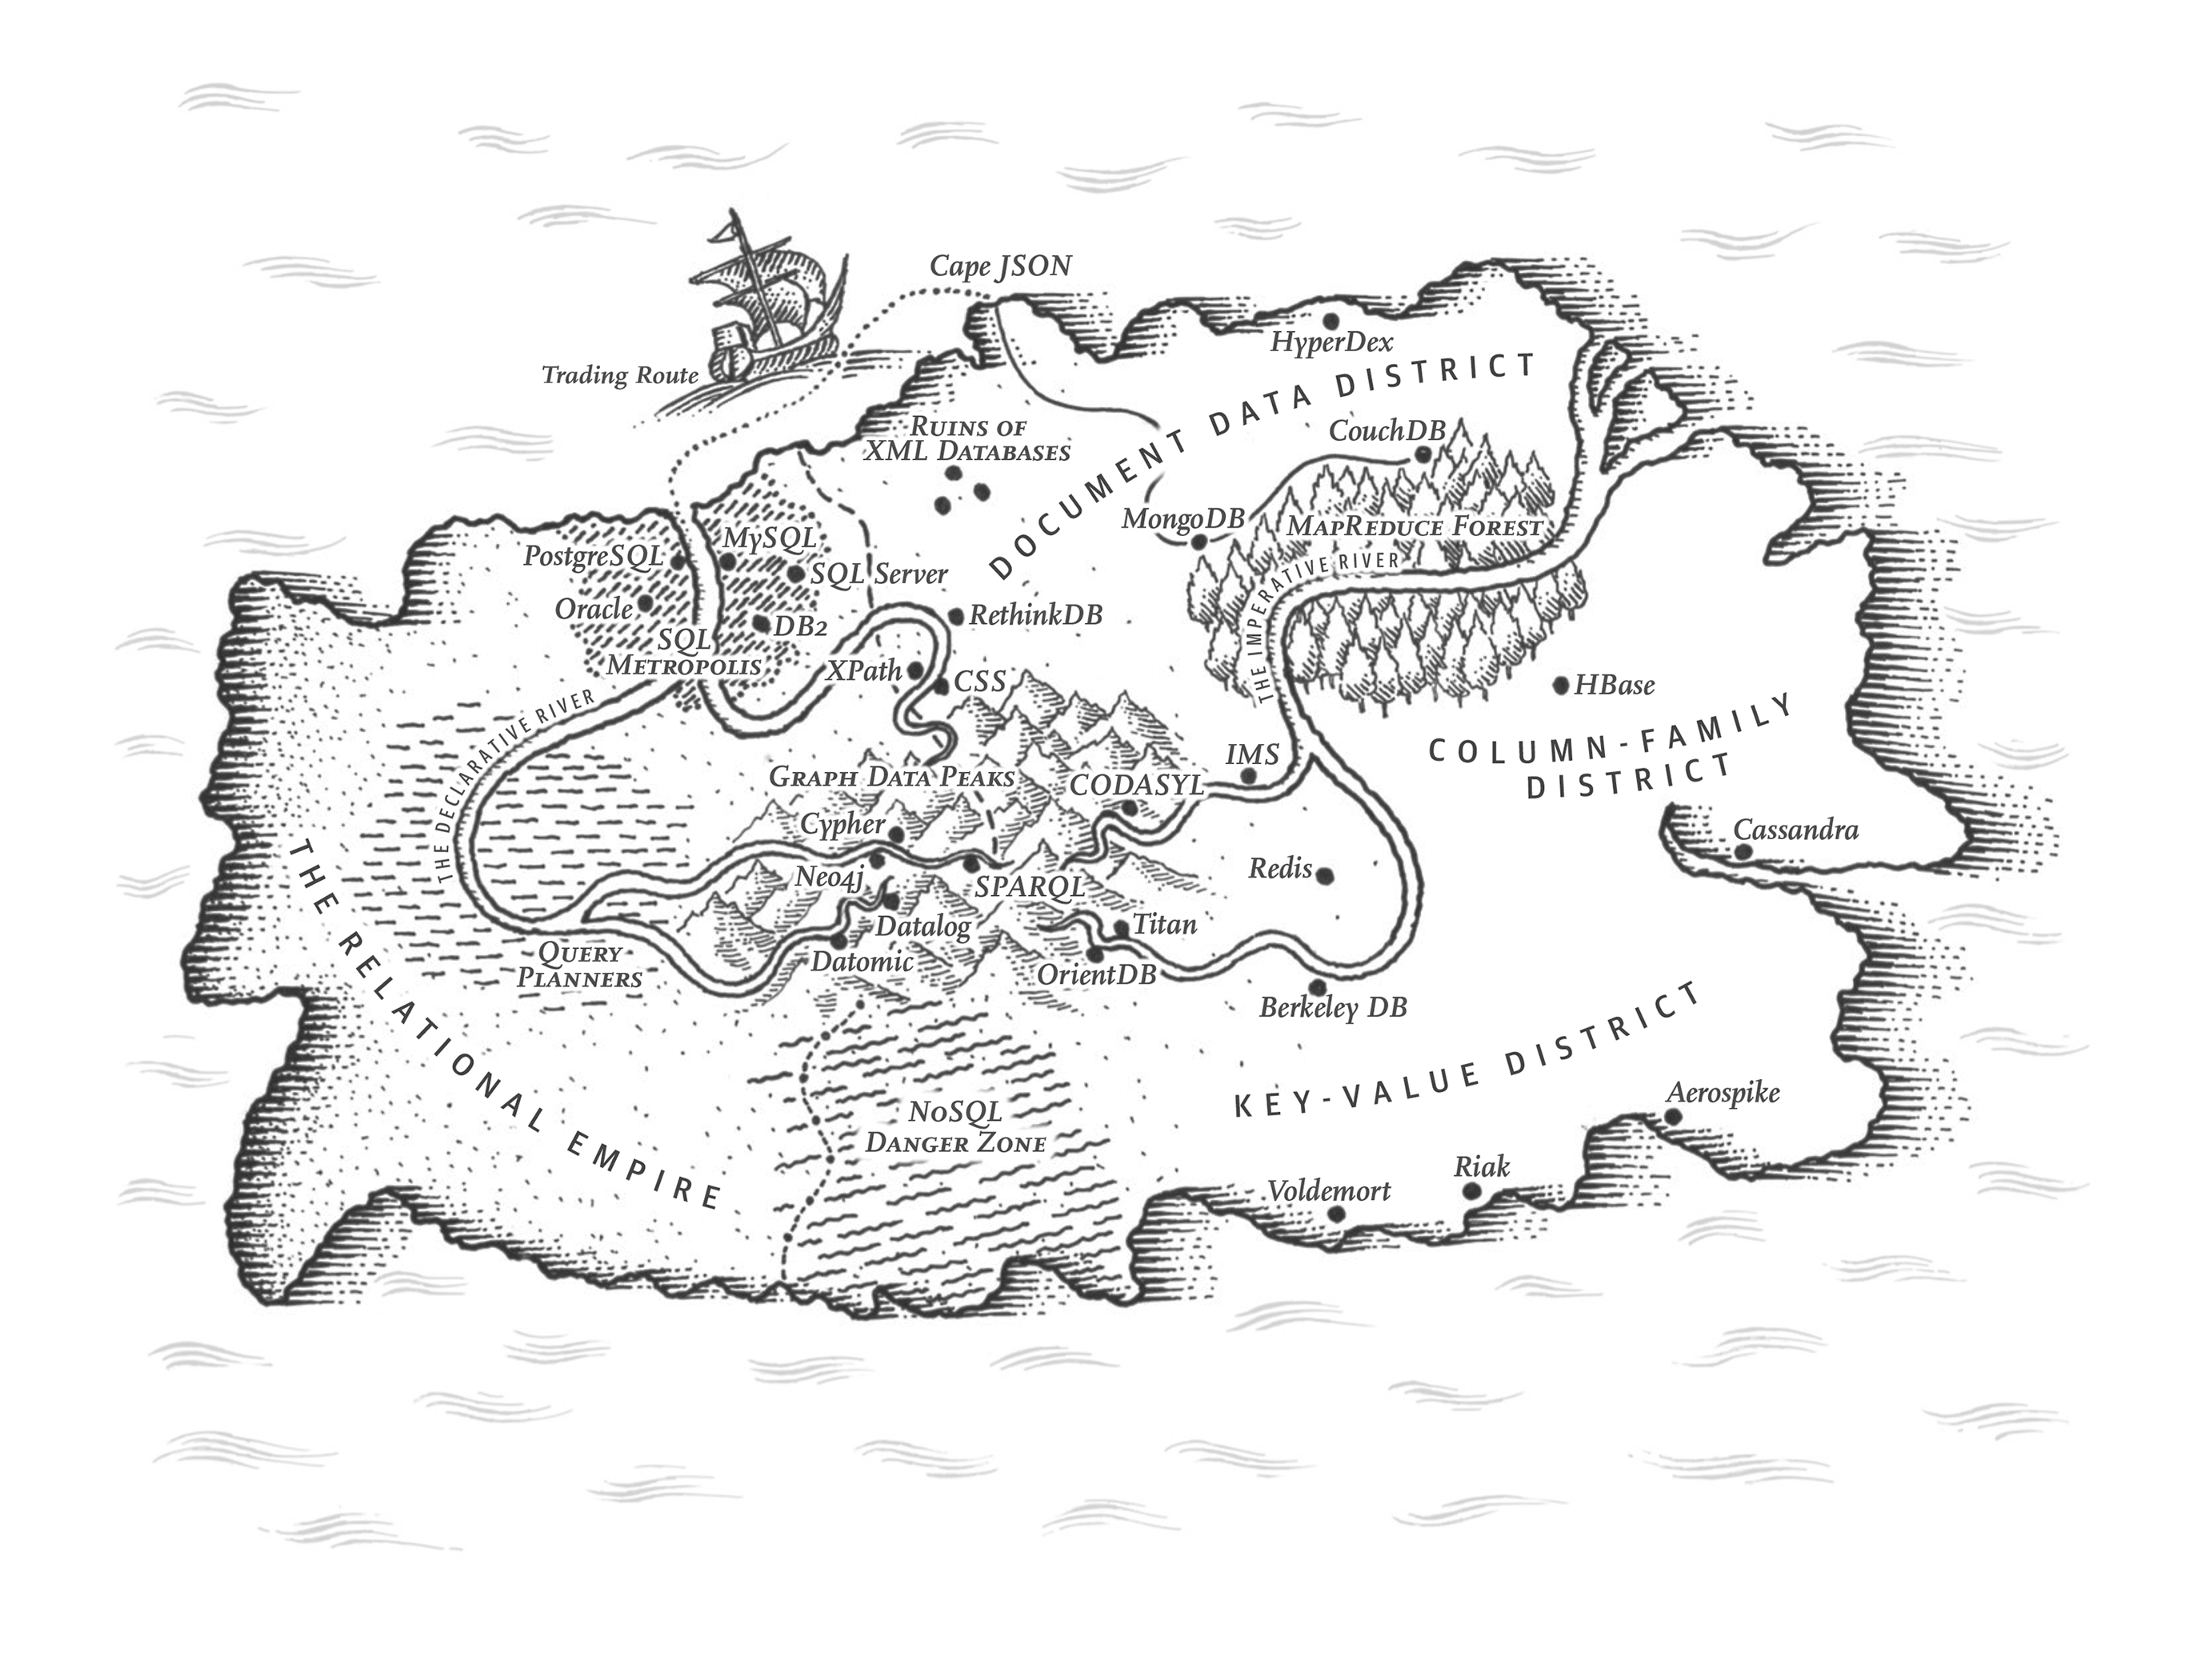
\includegraphics[width=\textwidth]{images/databases}
  }
\caption{A map of data storage techniques from Designing Data-Intensive Applications \cite{data-intensive}.}
\end{figure}

\section{This Week}
This week our goal is to:
\begin{itemize}
  \item explore the various techniques developers use to store data;
  \item investigate the storage options implementing these techniques on the AWS platform;
  \item upgrade our todo application to use a relationsal database.
\end{itemize}

\section{Databases and Data Models}
Unfortunately, to build interesting software we often need to store and use data.
The storage of data introduces a number of challenges when designing, creating, and maintaining our software.
However, not all data storage techniques are created equal;
the choice of data storage model can have a profound impact on our software's complexity and maintainability.
In this practical, we want to take a superficial exploration of our island of data storage models.
For a more in-depth treatment of data storage models that is outside the scope of this course,
see Chapter 2 of the \textit{Designing Data-Intensive Applications} book \cite{data-intensive}.

\teacher{
  Discuss the following different storage technologies and mention some use cases of when you would choose each one.
  Discuss some popular implementations of each.\\

  Aim for no more than 30 minutes of discussion.
}

\subsection{Relational Storage}

Relational databases what have been exposed to the most in your University career --- think MySQL, Postgres, Oracle DB, etc.
This type of database is good at modelling the real world which is often a highly connected environment.
% The data model that is suggested for this type of storage is a normalised approach where data duplication should be reduced.

Some popular offerings are below:

\begin{itemize}
  \item MySQL/MariaDB [ Amazon RDS / Amazon Aurora ].
  \item Postgres [ Amazon RDS / Amazon Aurora ].
\end{itemize}

The AWS offerings of these services come in two different types, we have the traditional approach of
server capacity ( x cores, y ram ) and we have a server-less approach.
The server-less approach is a more dynamic
database that can scale to large amounts of load when needed though at a cost per request.

  \subsubsection{ORM}
  Object Relational Mapping (ORM) is a fairly common tool for programmers to use to make developing with databases smoother.
  One fairly prevalent example of this is SQLAlchemy which is a very widely used 
  database abstraction for python.
  SQLAlchemy allows us to move to a higher level of abstraction than SQL queries and perform database actions using standard python code.

  The benefits of ORMs are the ability to model database objects in our existing programming language instead of having large blocks of SQL text within our source code.
  The disadvantages come in when we need to do specific SQL work or where the abstractions cost is greater than the benefits.

\subsection{Wide-Column Storage}

\teacher{
  Examples of big apps that depend on this technology is Netflix \url{https://netflixtechblog.com/netflixs-viewing-data-how-we-know-where-you-are-in-house-of-cards-608dd61077da}.
}

Wide-Column databases are a form of NoSQL or non-relational data stores.
In these data stores the data model design 
is focused more on having efficient queries at the cost of data duplication.
A warning to the reader that these models
are not flexible after creation, it is much easier to answer a new use case in a relational model.

  \begin{itemize}
    \item Apache Cassandra [ Amazon Keyspaces for Cassandra ].
    \item Apache HBase.
  \end{itemize}

\subsection{Key-Value Storage}

Key-Value stores are very popular for cache or remote config use cases, some of the most notable are Redis and Memcached.
These stores allow efficient lookup of values via keys and are usually stored in-memory.

\begin{itemize}
  \item Redis [ Amazon ElastiCache for Redis ].
  \item Memcached [ Amazon ElastiCache for Memcached].
  \item Amazon DynamoDB.
  \item Amazon MemoryDB for Redis.
\end{itemize}

\subsection{Time Series Storage}

\teacher{
  Something to mention here is that relations are usually not utilised between tables in time series databases.
}

Time series databases are highly focused storage which is tailored to retrieving results by timestamp ranges.
Many implementations also take advantage of the data model to allow efficient rollover of data and partitioning.
One of the most popular time series databases is Prometheus which is used to store monitoring metrics.

\begin{itemize}
  \item Amazon Timestream.
  \item TimescaleDB ( Postgres + Addon ).
  \item Prometheus.
  \item InfluxDB.
\end{itemize}

\subsection{Document Storage}

Document databases are a subset of NoSQL databases with a focus on a flexible data model.
MongoDB for instance allows the user to store JSON documents and perform queries on those documents.
One advantage of document databases is that they match a programmers existing mental model of storing data in formats such as JSON.

\begin{itemize}
  \item MongoDB.
  \item Apache CouchDB.
  \item Amazon DocumentDB.
  \item Amazon DynamoDB.
\end{itemize}

\subsection{Graph Storage}

\teacher{
  If you havnt experienced graph databases, a good usecase is ``recommendation systems'',
  which use the connected nature of items to figure out what to suggest to a person.Another example is the \url{https://neo4j.com/blog/analyzing-panama-papers-neo4j/}
  Panama Papers.
}

Graph Databases are relational storage with a few enhancements to allow fast neighbour look-ups.
These databases also allow the implementation of graph algorithms to query data.

\begin{itemize}
  \item Amazon Neptune.
  \item Neo4J.
  \item Janus Graph.
\end{itemize}

\section{Enhancing the Todo App with Storage}

\teacher{
  We will be using the todo app from the previous practical as a starting point.
  We will be adding a database to the application to store the todo items.
  We will be using a relational database to store the data.
  We will be using SQLAlchemy to abstract the database away from the application.
  We will be using Flask-Migrate to manage the database migrations.
}

\bibliographystyle{ieeetr}
\bibliography{books,ours}

\end{document}